\chapter{Behavioral Systems Theory}\label{ch:Behaviors}

The behavioral approach to systems theory, pioneered by Willems~\cite{willems2007}, offers a framework for modeling and analyzing dynamical systems based on their observed behaviors, rather than relying on explicit parametric models. In this chapter, we provide an overview of the key concepts in behavioral systems theory, including the definition of behaviors, the construction of Hankel matrices, and the fundamental lemma that underpins data-driven control methods.

\section{Behaviors}
In the behavioral framework, a dynamical system is characterized by its \emph{behavior}, which is defined as the set of all possible trajectories (input-output sequences) that the system can exhibit.

\subsection{Notation and terminology}

\subsubsection{Sets and functions}
The set of positive and non-negative integers are denoted by $\N$ and $\Z_+$, respectively. The set of real and non-negative real numbers are denoted by $\R$ and $\R_+$, respectively.  
For ${T\in\N}$, the set of integers $\{1, 2, \dots , T\}$ is denoted by $\mathbf{T}$.  A map $f$ from $X$ to $Y$ is denoted by ${f:X \to Y}$; $(Y)^{X}$ denotes the set of all such maps. The \textit{restriction} of ${f:X \to Y}$ to a set ${X^{\prime}}$, with ${X^{\prime} \cap X \neq \emptyset}$, is denoted by $f|_{X^{\prime}}$ and is defined by $f|_{X^{\prime}}(x)$ for ${x \in X^{\prime}}$; if ${\mathcal{F} \subseteq (Y)^{X}}$, then $\mathcal{F}|_{X^{\prime}}$ is defined as ${\{ f|_{X^{\prime}} \, : \, f \in \mathcal{F}\}}$.

\subsubsection{Linear algebra}
The transpose, image, and kernel of a matrix ${M\in\R^{m\times n}}$ are denoted by $M^{\top}$, $\Image\, M$, and $\Ker M$, respectively. The $m \times p$ zero matrix is denoted by $0_{m \times p}$ and the $m \times p$ matrix with ones on the main diagonal and zeros elsewhere is denoted by $I_{m \times p}$. For $m = p$, we use $0_p$ and $I_p$, and subscripts are omitted when dimensions are clear from context. The Kronecker product of the matrices $M \in \R^{m \times n}$ and $N \in \R^{p \times q}$ is denoted by $M \otimes N$. 


\subsection{Sequences, shift operator, Hankel matrices}

 A \textit{sequence} is a function ${w: S \to \R^q}$, where ${S \subseteq \N}$; the sequence is \textit{finite} if $S$ has finite cardinality, and \textit{infinite} otherwise. An infinite sequence ${w}$ is also denoted by $\{w_k\}_{k\in\N}$. We use the terms \textit{sequence}, \textit{time series}, and \textit{trajectory} interchangeably.  By a convenient abuse of notation, a finite sequence ${w\in(\R^q)}^\mathbf{T}$ is often identified with the corresponding column vector ${w=\col(w(1),\ldots,w(T))\in\R^{qT}}.$

The \textit{shift operator} ${\sigma : {(\R^q)}^\N \to {(\R^q)}^\N}$ is defined as
 \begin{equation}
    \sigma w (t)= w(t+1).
 \end{equation}

 By convention, the shift operator acts on all elements of a set ${\mathcal{W} \subseteq {(\R^q)}^\N}$, that is, $\sigma \mathcal{W}  =\{\sigma w\,:\, w\in\mathcal{W} \}$.

The \textit{Hankel matrix} of depth ${L\in\mathbf{T}}$ associated with the sequence ${w\in {(\R^q)}^\mathbf{T}}$ is defined as 
 \begin{equation} \label{eq:Hankel} 
 \mathcal{H}_{L}(w) =
 \begin{bmatrix}
    w(1) & w(2) & w(3) & \cdots & w(T-L+1) \\
    w(2) & w(3) & w(4) & \cdots & w(T-L+2) \\
    \vdots & \vdots & \vdots & \ddots & \vdots \\
    w(L) & w(L+1) & w(L+2) & \cdots & w(T)
 \end{bmatrix}
 \end{equation}

 \subsubsection{Systems}
 In behavioral systems theory~\cite{willemspolderman1998}, a \textit{system} is a triple $\Sigma=(\T,\W,\Be),$ where $\T$ is the \textit{time set}, $\W$ is the \textit{signal set}, and $\Be \subseteq (\W)^{\T}$ is the \textit{behavior} of the system. Throughout this work, we exclusively focus on \textit{discrete-time} systems, with ${\T = \N}$ and ${\W = \R^q}$. We adapt definitions accordingly, emphasizing this assumption when necessary. By a convenient abuse of notation, we also identify a system $\Sigma$ with the corresponding behavior $\Be$.

 \subsubsection{LTI systems}
 A system $\Be$ is \textit{linear} if $\Be$ is a linear subspace, \textit{time-invariant} if $\Be$ is shift-invariant, \textit{i.e.}, ${\sigma(\Be) \subseteq \Be}$, and \textit{complete} if ${w\in\Be}$ if and only ${w|_{[t_0,t_1]} \in \Be|_{[t_0,t_1]}}$ for every ${-\infty < t_0 \le t_1 < \infty}$. Completeness of a discrete-time linear system $\Be$ is equivalent  to $\Be$ being closed in the topology of pointwise convergence~\cite[Proposition 4]{willems1986}. The set of all (discrete-time) complete LTI systems is denoted by $\mathcal{L}^q$.  By a convenient abuse of notation, we often write $\Be \in \mathcal{L}^{q}$.


 \subsubsection{Kernel representations}
 Every LTI system ${\Be \in \mathcal{L}^{q}}$ admits a \textit{kernel representation} of the form
 \begin{equation}
 \Be = \Ker R(\sigma) ,
 \end{equation}
 where  $R(\sigma)$ is the operator defined by the polynomial matrix 
\[
R(z) = R_1 + R_2 z + \cdots + R_{d}z^{d-1},
\]
 with $R_i\in\R^{g\times q}$ for $i\in\text{\boldmath$d$\unboldmath},$ and 
 \[
   \Ker R(\sigma) = \{w\in{(\R^q)}^\N \,:\, R(\sigma)w = 0\}.
 \]
 Without loss of generality, one may assume that  $\Ker R(\sigma)$  is a \emph{minimal}  kernel representation of $\B$,  \textit{i.e.},  $R(\sigma)$ has full row rank~\cite{willems1989}.


 \subsubsection{Partitions}
 Given a permutation matrix ${\Pi\in\R^{q\times q}}$ and an integer $0 < m < q$, the map defined by the equation
 \begin{equation} \label{eq:partition} 
 (u,y) = \Pi w 
 \end{equation}
 induces a \textit{partition} of each ${w\in\R^q}$ into the variables ${u\in\R^m}$ and ${y\in\R^{q-m}}$.  For LTI systems, we can also simply identify trajectories as 
 \begin{equation} \label{eq:partition_lti}
   w = \begin{bmatrix}
      u \\
      y
   \end{bmatrix}
 \end{equation}
 We write $w \sim (u,y)$ if~\eqref{eq:partition} holds for some  permutation matrix ${\Pi\in\R^{q\times q}}$ and integer ${0 < m < q}$.  
 Any partition~\eqref{eq:partition} induces natural  projections  ${ \pi_u:  w \mapsto u}$ and ${ \pi_y:  w \mapsto y}$. We call~\eqref{eq:partition} a \textit{partition of ${\Be\in\mathcal{L}^{q}}$} if~\eqref{eq:partition} holds for all ${w\in\Be}$; the partition~\eqref{eq:partition} is an \textit{input-output partition} if $u$ is an \textit{input} and $y$ is an \textit{output} (see~\cite[p.568]{willems1986} for definitions).

 \subsubsection{Integer invariants}
 The structure of an LTI  system ${\Be \in\mathcal{L}^q}$ is characterized by a set of \textit{integer invariants}~\cite{willems1986}, defined as
 \begin{itemize}
 \item the \textit{number of inputs} ${m(\Be) = q-\text{row dim} R(\sigma)}$,  
 \item the \textit{number of outputs} ${p(\Be) = \text{row dim} R(\sigma)}$,  
 \item the \textit{lag} ${\ell(\Be) = \max_{i \in\mathbf{p}}\{\deg\text{row}_i R(\sigma) \}}$, and
 \item the \textit{order} ${n(\Be)=\sum_{i \in\mathbf{p}} \deg\text{row}_i R(\sigma) }$, % ${n=\ell_1+ \ldots+ \ell_p}$,
 \end{itemize}
 where   
 $\Ker R(\sigma)$  is a minimal  kernel representation of $\Be$, while   
 ${\text{row dim}R}$ and ${\deg\text{row}_i R}$ are the number of rows and the degree of the $i$-th row of $R(z)$, respectively. The integer invariants are intrinsic properties of a system, as they do not depend on its representation~\cite{willems1986}. Thus, we omit the dependence on the particular behavior if clear from context.


 \subsubsection{Latent variables} 
 A \textit{system with latent variables} is a tuple $\Sigma = (\N, \R^q, \R^\kappa, \Be_{\textup{full}})$, where $\N$ is the \textit{time set}, $\R^q$ is the set of \textit{manifest variables}, $\R^\kappa$ is the set of \textit{latent variables}, and $\Be_{\textup{full}} \subseteq (\R^q \times \R^\kappa)^{\N}$ is the \textit{full behavior}, respectively. The \textit{manifest behavior} of the system is defined as
 \begin{equation}
 \Be_{\textup{man}} = \{ w \in (\R^q)^\N \mid \exists \, \eta\in(\R^\kappa)^\N \text{ s.\,t. } (w, \eta) \in \Be_{\textup{full}} \},
 \end{equation}
 where $w$ is the \textit{manifest variable} and $\eta$ is the \textit{latent variable}. Manifest variables are \textit{external} and directly observable (e.g., inputs and outputs); latent variables are \textit{internal} (e.g., state and interconnection variables) and usually play an auxiliary~role.


 \subsubsection{State-space representations}
 Every finite-dimensional LTI dynamic system ${\B \in \mathcal{L}^{q}}$ can be described by the equations
 \begin{equation} \label{eq:state-space}
 \sigma x = Ax + Bu, \quad y=Cx+Du,
 \end{equation}
 and admits a (\textit{minimal}) \textit{input/state/output representation} 
 \begin{equation} \label{eq:partition-ISO} 
 \!  \! \Be \!  = \!
 \left\{  (u,y) \sim w \in (\R^{q})^\N \,:\, \exists \,x\in(\R^n)^{\N} \, \textup{s.t.}~\eqref{eq:state-space}~\text{holds}
 \right\},
 \end{equation}
 where
 \[
    \begin{bmatrix}
    A & B \\
    C & D
    \end{bmatrix} \in \R^{(n+p)\times (n+m)}
 \]
   and  $m$, $n$, and $p$ are the number of inputs, the order, and the number of outputs of $\Be$, respectively. State-space representations define systems where the latent variable is the state $x$.

\subsubsection{Data-driven representations}
 
Data-driven representations connect data directly to system behavior using data matrices. The restricted behavior of a finite-dimensional,  discrete-time, LTI system is a subspace, whose dimension is determined only by the integer invariants and time horizon.


 \begin{lemma}\cite[Lemma 2.1]{dorfler2022} \label{lemma:subspace}
 Let ${\Be \in \mathcal{L}^{q}}$ and ${L\in\N}$. The restricted behavior $\Be|_{[1,L]}$ is a subspace of $(\R^{q})^{\mathbf{L}}$ and ${\dim \Be|_{[1,L]}  =  m(\Be) L+ n(\Be)}$ for all ${L>\ell(\Be)}$. 
 \end{lemma}

As a direct consequence of Lemma~\ref{lemma:subspace}, the restricted behavior of a finite-dimensional, discrete-time,  LTI system can be represented as the image of a raw data matrix. Next, we summarize a version of this principle known as the \textit{fundamental lemma}~\cite{willems2005}.

\begin{lemma}~\cite[Corollary 19]{markovsky2020} \label{lemma:fundamental_generalized}
 Let ${\Be \in \mathcal{L}^{q}}$ and ${w \in \Be|_{[1,T]}}$. Fix $L\in\mathbf{T}$, with ${L > \ell(\Be)}$. Then  $\Be|_{[1,L]} = \Image  \mathcal{H}_L(w)$  if and only if
 \begin{equation}  \label{eq:generalized_persistency_of_excitation} 
 \rank  \mathcal{H}_L(w)   =  m(\Be)L+ n(\Be).
 \end{equation}
 \end{lemma}

\noindent
The rank condition~\eqref{eq:generalized_persistency_of_excitation} is referred to as the  \emph{generalized persistency of excitation} condition~\cite{markovsky2020}. Thus, we call a trajectory ${w \in \Be|_{[1,T]}}$ of a system ${\Be \in \mathcal{L}^{q}}$ \emph{generalized persistently exciting (GPE) of order $L$} if~\eqref{eq:generalized_persistency_of_excitation} holds. Different variations of this principle can be formulated under a range of assumptions, see, \textit{e.g.}, the recent survey~\cite{markovsky2021} for an overview and~\cite{padoan2022} for some extensions to broader classes of systems.

\newpage
\section{System Identification}

System identification in the behavioral framework involves constructing a behavior $\Be$ that accurately captures the dynamics of a system based on observed data. 

Using the fundamental lemma (Lemma~\ref{lemma:fundamental_generalized}), one can identify the behavior of a finite-dimensional, discrete-time, LTI system from a set of GPE trajectories. Specifically, given a set of trajectories ${\{w_i\}}_{i=1}^{T_d}$ that are GPE of order $L$, the restricted-behavior can be reconstructed as
\begin{equation}
   \Image \mathcal{H}_L(w) = \Be_{[1,L]}
\end{equation} 

\subsection{Effect of noise}
In practical scenarios, data is often corrupted by noise, which can affect the accuracy of (behavioral) system identification. The rank of the Hankel matrix may be inflated due to noise, masking the system's actual order. To mitigate this, techniques such as singular value decomposition (SVD) can be employed to approximate the Hankel matrix and extract the dominant dynamics.

The singular values of the Hankel matrix can provide insights into the underlying system order, allowing for a more robust identification process in the presence of noise. An analysis of the magnitude of singular values for noisy data and ideal data is shown in Figure~\ref{fig:svd_noise}, which was performed for a simple SISO system (double integrator) with $10\%$ additive Gaussian noise. It can be observed that the presence of noise inflates the singular values, masking the true system order. The noise floor, indicated by the dashed line, is where the singular values suddenly drop off, suggesting a cutoff for identifying the system order in the ideal case.

\begin{figure}[h]
      \centering
      \includegraphics[width=\textwidth]{figures/noise_floor.png}
      \caption{Singular values of Hankel matrices constructed from ideal data (blue) and noisy data (red). The noise floor is shown by the dashed line.}
      \label{fig:svd_noise}
\end{figure}

\subsection{Grassmannians and Behaviors}
Behaviors can be viewed as points on a Grassmannian manifold, which is the space of all $k$-dimensional subspaces of an $n$-dimensional vector space. This perspective allows for the application of geometric methods in system identification and analysis.

Given restricted behavior $\Be|_{[1,L]}$ of dimension $k = m(\Be)L + n(\Be)$, we can associate it with a point on the Grassmannian manifold $\Gr(k, qL)$.

Denote $r_H = \rank \mathcal{H}_L(w)$ for trajectories ${\{w_i\}}_1^{T_d}$. Depending on the noise level, $r_H$ satisfies the following:
\begin{equation}
  k \leq r_H \leq n,
\end{equation}
where $n = qL, k = m(\Be)L + n(\Be)$. Still, only the first $k$ singular vectors of $\mathcal{H}_L(w)$ correspond to the behavior $\Be$. Thus, the behavior can be identified with a point on the Grassmannian manifold $\Gr(k, n)$. To obtain an orthonormal basis for the behavior, we can perform an SVD on $\mathcal{H}_L(w)$ and extract the first $k$ left singular vectors. This basis spans the same subspace as $\Be|_{[1,L]}$, providing a representation of the behavior in the presence of noise. Thus,
\begin{equation}
   \mathcal{H}_L(w) = U \Sigma V^\top,
\end{equation}
where $U \in \R^{n \times r_H}$, $\Sigma \in \R^{r_H \times r_H}$, and $V \in \R^{(T_d-L+1) \times r_H}$. The first $k$ columns of $U$, is equivalently denoted by $\hat{Y}$ such that
\begin{equation}
   \hat{Y} \equiv U_{[1:k]},
\end{equation}
where $\hat{Y} \in \R^{n \times k}$ and $\hat{Y}^\top \hat{Y} = \I_k$. The subspace spanned by the columns of $\hat{Y}$ corresponds to the behavior $\Be|_{[1,L]}$, is also identified by $\hat{S} \in \Gr(k,n)$.

\subsubsection{Summary}
\begin{figure}[h]
   \centering
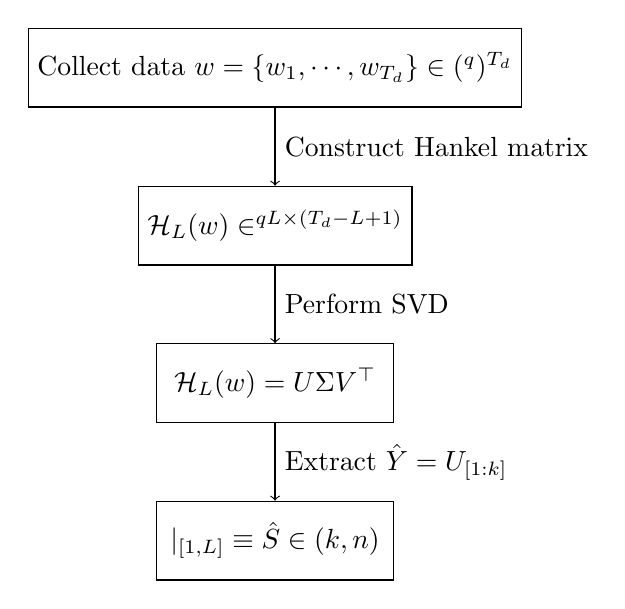
\begin{tikzpicture}[scale=0.6]
   \node (data) [draw, rectangle, minimum width=3cm, minimum height=1cm] {Collect data $w = \{w_1, \cdots, w_{T_d}\} \in {(\R^{q})^{T_d}}$};
   \node (hankel) [draw, rectangle, minimum width=3cm, minimum height=1cm, below=1.5cm] { $\mathcal{H}_L(w) \in \R^{qL \times (T_d-L+1)}$};
   \node (svd) [draw, rectangle, minimum width=3cm, minimum height=1cm, below=3.5cm] {$\mathcal{H}_L(w) = U \Sigma V^\top$};
   \node (grassmannian) [draw, rectangle, minimum width=3cm, minimum height=1cm, below=5.5cm] {$\Be|_{[1,L]} \equiv \hat{S} \in \Gr(k,n)$};
   \draw[->] (data) -- (hankel) node[midway, right] {Construct Hankel matrix};
   \draw[->] (hankel) -- (svd) node[midway, right] {Perform SVD};
   \draw[->] (svd) -- (grassmannian) node[midway, right] {Extract $\hat{Y} = U_{[1:k]}$};
\end{tikzpicture}
\end{figure}




